
  
  

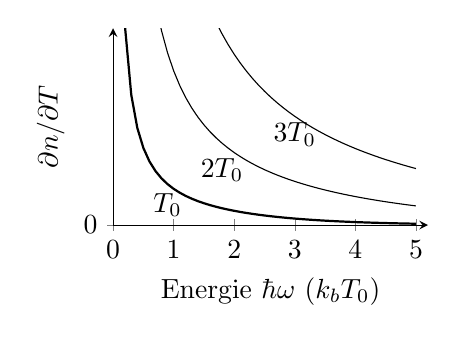
\begin{tikzpicture}

%\omega^2 =  \frac{c}{\mu}
%\pm c \sqrt{ \frac{1}{\mu^2} - \frac{4}{M_1 M_2}  \sin^2 \left( %\frac{1}{2}  \mathbf{k} \cdot \mathbf{a} \right) } 


%\useasboundingbox (0,0) rectangle (5,5);
%\draw (0,0) rectangle (5,5);



\begin{axis}[%clip=false ,
    height=2.5cm,
    width=4cm,
    xtick pos = bottom,
    scale only axis,
            separate axis lines,
  axis x line=bottom,
  axis x line shift=0pt,
  %xlabel shift=10pt,
  axis y line=left,
  axis y line shift=0pt,
%  ylabel shift=10pt    
 xlabel = {Energie $\hbar \omega$  ($k_b T_0$)}, 
ylabel = { $\partial \braket{n}  / \partial T$},
  axis y line=left, clip=true,
  xmin = 0, xmax = 5.2,
  ymin = 0, ymax = 5,
  ytick = {0},
  xtick = {0,1,2,3,4,5},
%,ytick pos = left, ytick = {0}, 
% xmin=1320, xmax = 1520, xtick = {1415}, xticklabel = {1415}
 ]

           

\addplot[thick, domain=0.1:5,samples=50]  {x * exp(x) / (exp(x) -1)^2};
\addplot[thin, domain=0.1:5,samples=50]  {x * exp(x/2) / (exp(x/2) -1)^2};
\addplot[thin, domain=0.1:5,samples=50]  {x * exp(x/3) / (exp(x/3) -1)^2};
 
\node at (0.9, 0.5) {$T_0$};
\node at (1.8, 1.4) {$2 T_0$};
\node at (3, 2.3) {$3 T_0$};

 \end{axis}

\end{tikzpicture}


